% Metódy inžinierskej práce

\documentclass[10pt,twoside,slovak,a4paper]{article}

\usepackage[slovak]{babel}
%\usepackage[T1]{fontenc}
\usepackage[IL2]{fontenc} % lepšia sadzba písmena Ľ než v T1
\usepackage[utf8]{inputenc}
\usepackage{graphicx}
\usepackage{url} % príkaz \url na formátovanie URL
\usepackage{hyperref} % odkazy v texte budú aktívne (pri niektorých triedach dokumentov spôsobuje posun textu)

\usepackage{cite}
%\usepackage{times}

\pagestyle{myheadings}

\title{Nástroje CASE a ich využitie v reverznom inžinierstve\thanks{Semestrálny projekt v predmete Metódy inžinierskej práce, ak. rok 2021/22 vedenie: Vladimír Mlynarovič}} % meno a priezvisko vyučujúceho na cvičeniach

\author{Šimon Ukuš\\[2pt]
	{\small Slovenská technická univerzita v Bratislave}\\
	{\small Fakulta informatiky a informačných technológií}\\
	{\small \texttt{xukus@stuba.sk}}
	}

\date{\small 4. november 2021} 



\begin{document}

\maketitle

\begin{abstract}
Článok sa zaoberá problematikou softvérového inžinierstva, kontkrétne ako je možné proces vývoja softvéru automatizovať pomocou nástrojov CASE - Computer-Aided Software Engineering (Počítačom podporované softvérové inžinierstvo). V práci sa popisuje či už delenie týchto nástrojov,  tak aj sféry ich využitia.  Článok ďalej skúma softvérové inžinierstvo a použitie CASE nástrojov z inej perspektívy.  Na rozdiel od vnímania vývoja softvéru klasicky, teda smerom vpred (Forward Engineering) sa venuje tzv. spätnému inžinierstvu (Reverse Engineering). Tu je skúmaná kompletnosť a presnosť spätne navrhnutých UML diagramov generovaných nástrojmi CASE. Predmetom porovnania bolo celkom 8 nástrojov (z toho 6 open source a 2 komerčné). Tieto nástroje boli hodnotené na základe toho, aké typy vstupov podporujú, aké typy diagramov dokážu rekonštruovať a v akej kvalite.
 
\end{abstract}



\section{Úvod}
Pojem softvérové inžinierstvo môže byť chápaný ako uplatňovanie metód, postupov a nástrojov na riadenie a vývoj počítačových systémov~\cite{1985}. Ide o komplexný postup, na ktorom sa zúčastňuje mnoho odborníkov z rôznych oblastí, ako napríklad projektový manažér, team líder, softvérový developer, tester, UI dizajnér a mnoho ďalších. Časť ich práce je možno automatizovať či uľahčiť využitím nástrojov CASE. Tieto nástroje sú špeciálne vyvinuté pre podporu vývoja softvéru, automatizujú proces vývoja. Cieľom ich implementácie je ušetrenie času a nákladov pri vývoji softvéru a zvýšenie jeho kvality~\cite{Osama:Adoption}.

Využitie nástrojov CASE a ich klasifikácia sú uvedené v časti~\ref{typy CASE}. V tejto časti je popísané delenie podľa toho, ktorú časť tzv. životného cyklu vývoja softvéru (Software Development Life Cycle, ďalej len SDLC) pomájhajú automatizovať. 
V časti~\ref{forward vs reverse} sa čitateľ zoznámi s pojmom \emph{reverzné inžinierstvo}. Nachádza sa tu prehľad, v ktorom je popísaný rozdiel medzi tzv. \emph{forward} (dopredným) a \emph{reverse} (spätným) inžinierstvom. 
Samotným nástrojom, ich predstaveniu a následnému porovnaniu sa venujú časti~\ref{predstavenie}~a~\ref{porovnanie}.
Záverečné hodnotenie týchto nástrojov prináša časť~\ref{zhrnutie}.



\section{klasifikácia nástrojov CASE a sféry použitia}\label{typy CASE}

Nástroje CASE sú odpoveďou na stále sa narastujúce nároky a zvyšujúcu sa komplexnosť počítačových systémov. Podporujú vývoj softvéru a dajú sa aplikovať v niektorých, niekedy vo všetkých fázach SDLC, ktorého podpora je čoraz žiadúcejšia. Náklady na vývoj softvéru každým rokom vzrastajú a preto čo i len skromné vylepšenia pri vývoji a automatizácii môžu znamenať veľké úspory.  Sú cielené na riešenie ťažkostí pri vývoji vysokokvalitného a komplexného softvéru načas a v súlade s rozpočtom~\cite{2001}.
\subsection{Klasifikácia nástrojov CASE}\label{klasifikácia}
Ako sa vyššie spomína, nástroje CASE slúžia na podporu rôznych fáz SDLC, prípadne dokážu automatizovať všetky z nich. Zvyknú sa preto klasifikovať podľa toho, ktoré štádium životného cyklu podporujú. Takéto rozdelenie vyzerá nasledovne:

\begin{itemize}
\item Upper CASE nástroje
\item Lower CASE nástroje
\item Integrated CASE nástroje
\end{itemize}
\textbf{Upper CASE}, niekedy označované aj ako \emph{front end CASE} slúžia na podporu skorých fáz životného cyklu softvéru, napríklad pri analýze a dizajne.\\
\textbf{Lower CASE}, tiež nazývané aj \emph{back end CASE} zase nachádzajú využitie pri neskorších fázach životného cyklu softvéru, najmä pri testovaní a vytváraní kódu.\\
\textbf{Integrated CASE}, sú schopné pokryť obe časti SDLC~\cite{1998}.


Iný pohľad na kategorizáciu poskytuje autor~\cite{2017}, ktroý nespája fázy SDLC do tzv. skorých a neskorších, ale konkrétne fázy jednotlivo vymenúva a podľa toho delí nástroje CASE delí nasledovne.
\begin{itemize}
\item Nástroje na riadenie projektov
\item Nástroje na analýzu a návrh
\item Nástroje na podporu Objektovo-Orientovaného softvérového inžinierstva
\item Nástroje na testovanie
\item Nástroje formálnych metód
\item Klient/Server nástroje
\item Nástroje pre webové inžinierstvo
\item Nástroje na opätovné inžinierstvo (Reengineering)
\end{itemize}

Pri tomto delení sa stretávame s pojmom opätovné inžinierstvo (Reengineering) a keďže v ďalších kapitolách je rozpracovaná téma reverzného inžinierstva a použitie nástrojov CASE v reverznom (spätnom) inžinierstve, je potrebné uviesť, že je rozdiel medzi spätným inžinierstvom (Reverse Engineering) a opätovným inžinierstvom (Reengineering). Síce oba pojmy odkazujú na ďalšie skúmanie alebo vývoj už hotových produktov, metódy a požadované výsledky sa výrazne líšia.  Ako~\cite{reengineering} ďalej vysvetľuje, reverzné inžinierstvo sa snaží odhaliť, ako daný systém funguje. Kdežto na druhej strane úlohou opätovného inžinierstva je zlepšenie súčasného návrhu skúmaním jeho konkrétnych aspektov. 

\subsection{Sféry použitia nástrojov CASE}\label{sféry}
\emph{//rozpracovaná kapitola, zatiaľ prázdna, neskôr pridám text.}

\section{Z dopredného inžinierstva k spätnému}\label{forward vs reverse}
\begin{figure}[tbh]
\centering
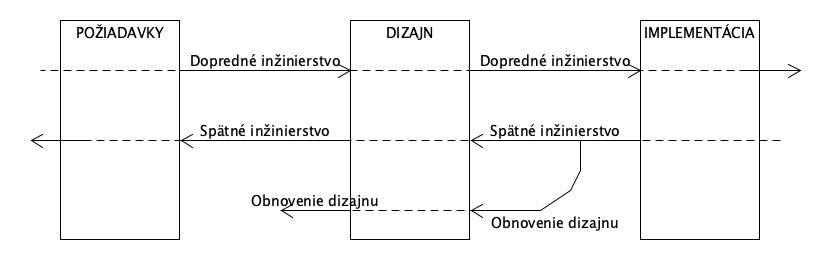
\includegraphics[width=0.85\textwidth]{forward_reverse.jpg}
\caption{Niektoré fázy SDLC a znázornené procesy súvisiace s dopredným a spätným inžinierstvom \cite{2010}}
\label{obr_forward_reverse}
\end{figure}

Spätné inžinerstvo, ako už bolo v sekcii~ \ref{klasifikácia} spomenuté, sa snaží pochopiť funkciu systému. Obr. \ref{obr_forward_reverse} ilustruje spôsob vývoja informačných systémov. Pre jednoduchosť boli použité tri fázy životného cyklu, kde prvá \emph{požiadavky} predstavuje špecifikáciu problému, druhá \emph{dizajn} zase špecifikáciu riešenia a tretia -  \emph{implementácia} predstavuje programovanie a testovanie požadovaného systému.

Dopredné \textit{(forward)} inžinierstvo predstavuje tradičný proces vývoja softvéru, kedy sa postupuje od prvotných abstraktných modelov, cez dizajn až ku konečnej implementácii systému. Môže sa zdať zbytočné, možno aj mätúce zavedenie názvu pre niečo tak priamočiare. V našom prípade, a tiež v mnoho iných, je to však nevyhnutné pre jeho odlíšenie od spätného inžinierstva. Ako teda Obr \ref{obr_forward_reverse} ukazuje, dopredné inžinierstvo prechádza jednotlivými fázami SDLC z ľava do prava.

// Tu príde ešte popis reverzného inžinierstva spolu s odkazovaním sa na obrázok.
\section{Predstavenie nástrojov}\label{predstavenie}

\section{Porovnanie nástrojov}\label{porovnanie}

\section{Zhrnutie} \label{zhrnutie} 




%\acknowledgement{Ak niekomu chcete poďakovať\ldots}


% týmto sa generuje zoznam literatúry z obsahu súboru literatura.bib podľa toho, na čo sa v článku odkazujete
\bibliography{literatura}
\bibliographystyle{abbrv} % prípadne alpha, abbrv alebo hociktorý iný
\end{document}
